%   The deposited PDF sets the appendix as an unnumbered-chapter section, which
%   is why its heading reads ".1" and its figures are numbered 5, 6, ... without
%   a chapter prefix. Reproduced as printed.

\renewcommand{\thefigure}{\arabic{figure}}
\setcounter{figure}{4}
\section{Appendix of Figures}
\clearpage

\begin{figure}[p]
\centering
\begin{subfigure}{\linewidth}\centering
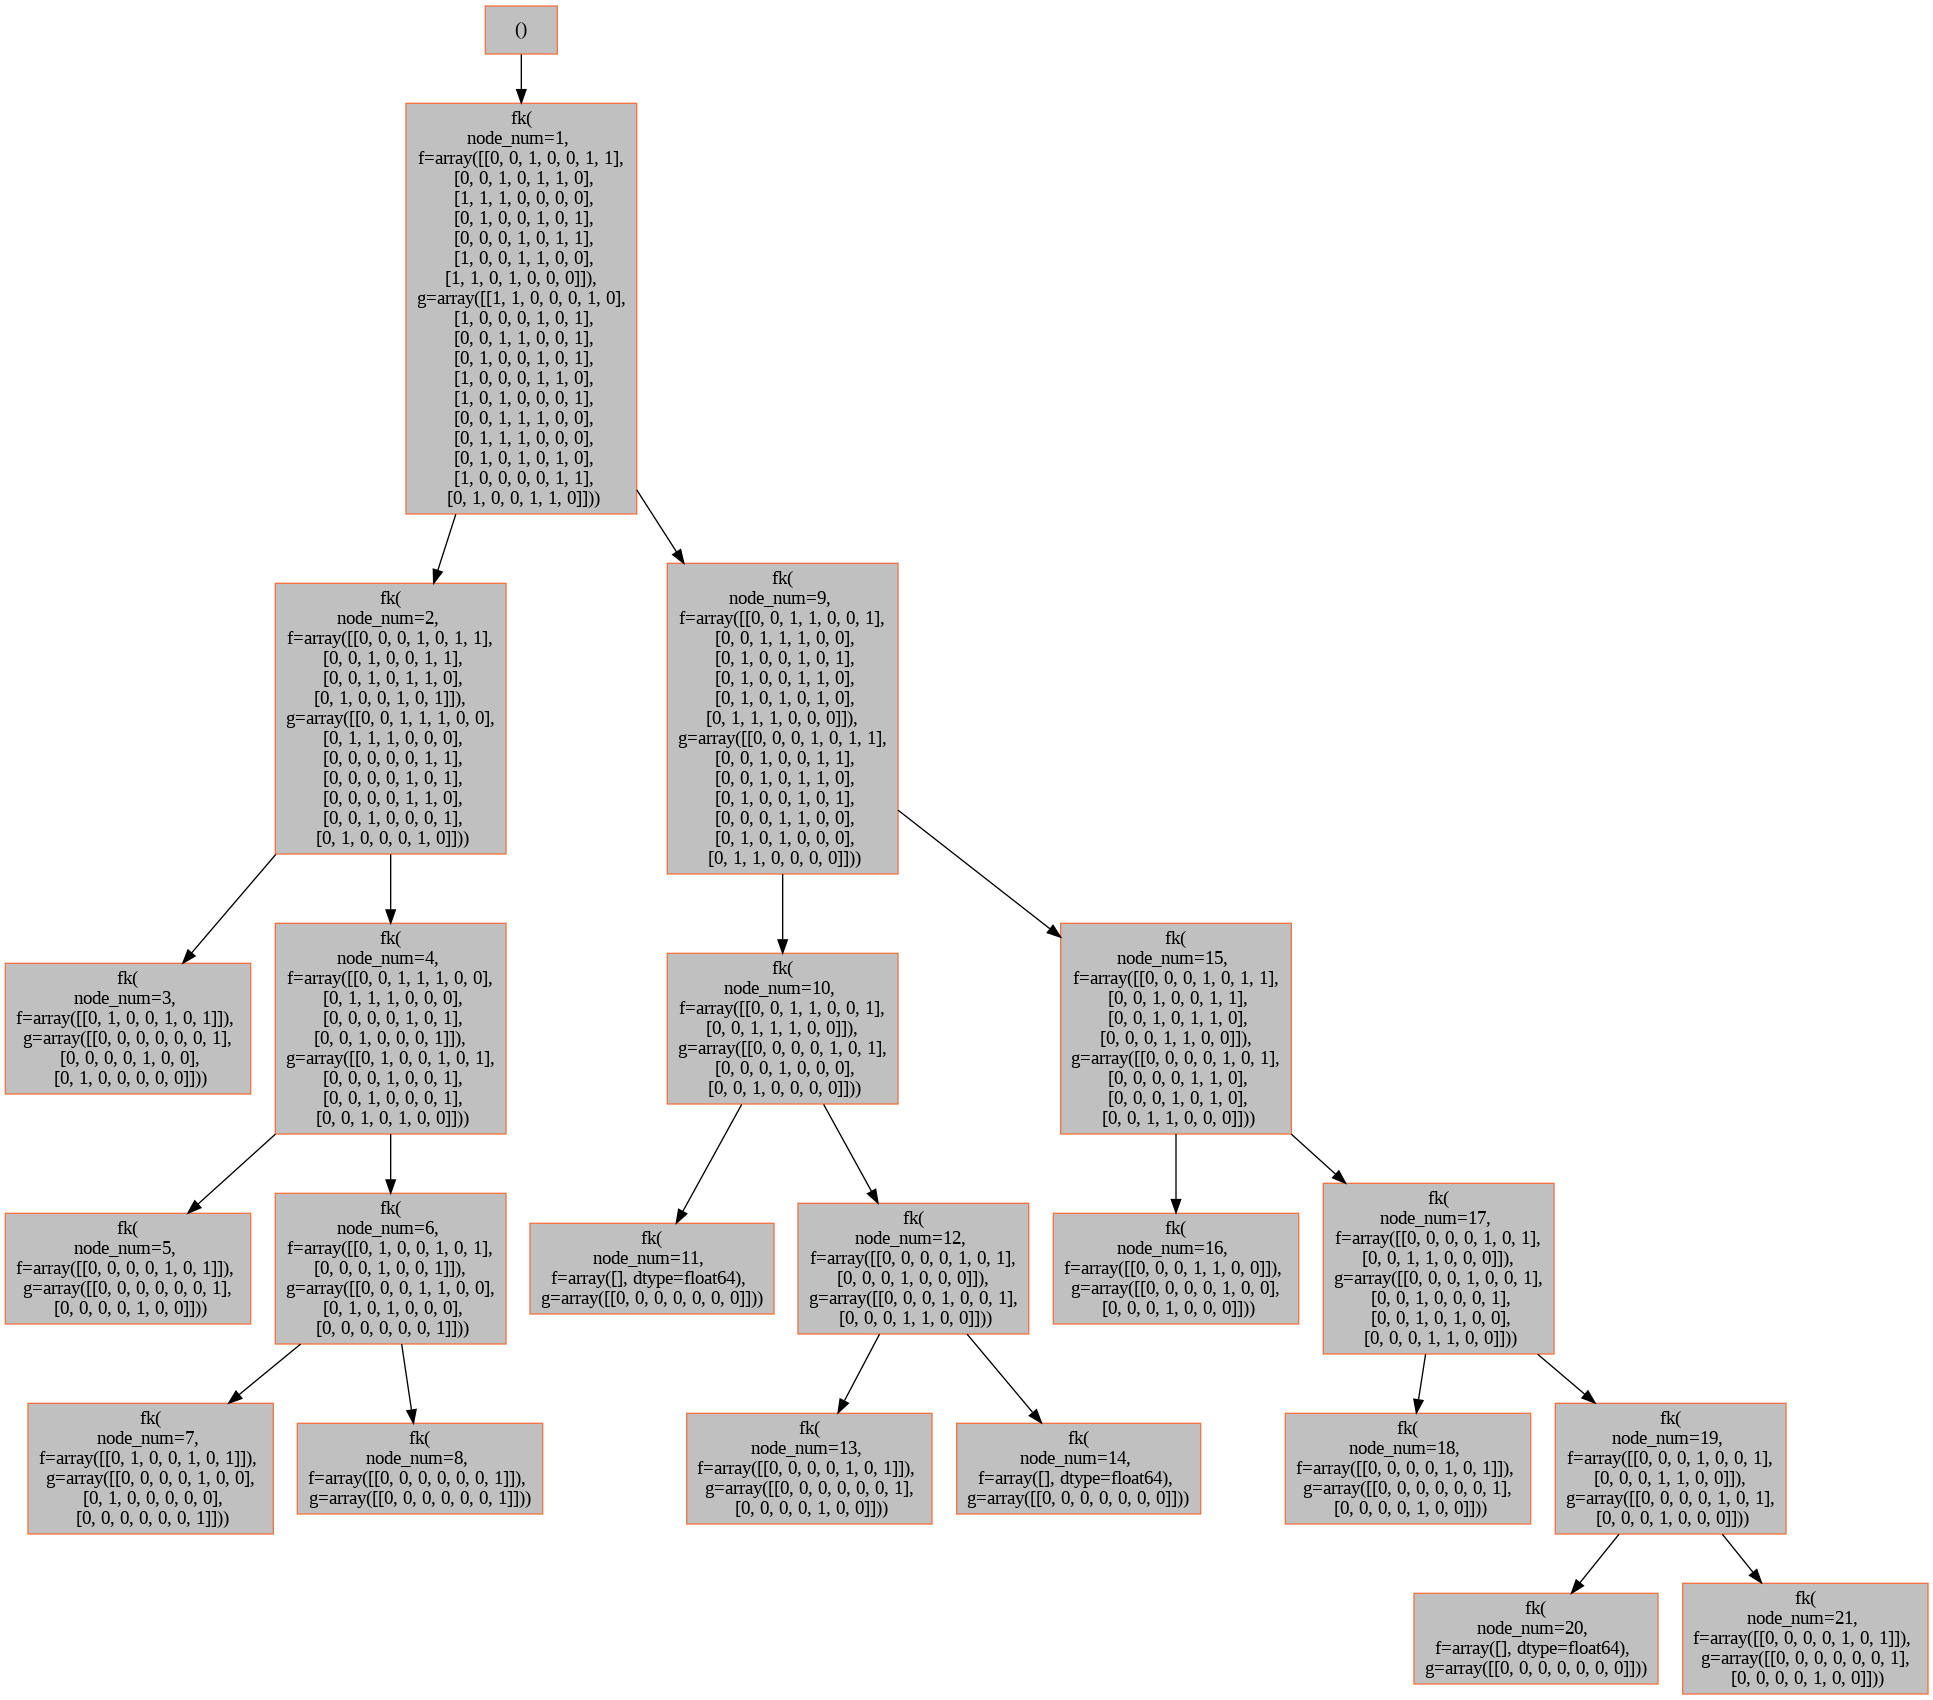
\includegraphics[width=0.62\linewidth]{figures/7ver-fka.png}
\caption{Visualization of 7-vertex Hypergraph in \FKA}
\end{subfigure}\\[4pt]
\begin{subfigure}{\linewidth}\centering
\resizebox{0.9\linewidth}{!}{\begin{forest}
autotree
[{\anode{1}{$v_{1}$}{$C_2$}{}{Cograph}}
  [{\anode{2}{$v_{6}$}{$\text{Trivial}$}{Non-Conformal}{Split, Chordal}}
    [{\anode{3}{}{$C_3$}{}{}}]
    [{\anode{4}{$v_{3}$}{$\text{Trivial}$}{Non-Conformal}{Split, Chordal, Cograph}}
      [{\anode{5}{}{$C_2$}{}{}}]
      [{\anode{6}{$v_{4}$}{$C_2$}{Read-Once, $\alpha$-acyclic}{}}
        [{\anode{7}{}{$C_3$}{}{}}]
        [{\anode{8}{}{$C_1$}{}{}}]
      ]
    ]
  ]
  [{\anode{9}{$v_{2}$}{$\text{Trivial}$}{Non-Conformal}{Split, Chordal, Cograph}}
    [{\anode{10}{$v_{3}$}{$C_2\times C_2$}{Read-Once, $\alpha$-acyclic}{Split}}
      [{\anode{11}{}{$\{\}$}{}{}}]
      [{\anode{12}{$v_{4}$}{$C_2$}{}{}}
        [{\anode{13}{}{$C_2$}{}{}}]
        [{\anode{14}{}{$\{\}$}{}{}}]
      ]
    ]
    [{\anode{15}{$v_{6}$}{}{$\alpha$-acyclic}{Bipartite}}
      [{\anode{16}{}{$C_2$}{}{}}]
      [{\anode{17}{$v_{3}$}{$D_8$}{}{$C_4$}}
        [{\anode{18}{}{$C_2$}{}{}}]
        [{\anode{19}{$v_{4}$}{$C_2$}{}{}}
          [{\anode{20}{}{$\{\}$}{}{}}]
          [{\textbf{Node: 21}\\Split vert.: $C_2$\\Hyp.:\\Graph:}]
        ]
      ]
    ]
  ]
]
\end{forest}
}
\caption{Automorphism Tree of 7-ver Hypergraph in \FKA}
\end{subfigure}
\caption{\FKA{} recursion tree and automorphism tree of 7-Ver. Hypergraph}
\end{figure}

\begin{figure}[p]
\centering
\begin{subfigure}{\linewidth}\centering
\resizebox{0.75\linewidth}{!}{\begin{forest}
autotree
[{\anode{1}{$v_{1}$}{$C_2\times D_4$}{Conformal (transversal not)}{}}
  [{\anode{2}{$v_{2}$}{$D_4$}{Conformal}{Chordal Bipartite}}
    [{\anode{3}{}{$S_3$}{}{}}]
    [{\anode{4}{$v_{6}$}{$D_4$}{Conformal}{Chordal Bipartite}}
      [{\anode{5}{$v_{5}$}{$C_2$}{}{}}
        [{\anode{6}{}{$\{\}$}{}{}}]
        [{\anode{7}{}{$C_2$}{}{}}]
      ]
      [{\anode{8}{}{$S_3$}{}{}}]
    ]
  ]
  [{\anode{9}{$v_{4}$}{$D_4$}{Conformal}{}}
    [{\anode{10}{$v_{3}$}{$C_2\times S_4$}{Read-Once, $\alpha$-acyclic}{}}
      [{\anode{11}{}{$\{\}$}{}{}}]
      [{\anode{12}{$v_{5}$}{$S_4\text{ (Non-terminal)}$}{Read-Once, $\alpha$-acyclic}{}}
        [{\anode{13}{}{$S_4$}{}{}}]
        [{\anode{14}{}{$\{\}$}{}{}}]
      ]
    ]
    [{\anode{15}{$v_{2}$}{$D_4$}{$\alpha$-acyclic}{}}
      [{\anode{16}{}{$S_3$}{}{}}]
      [{\anode{17}{$v_{6}$}{$C_2$}{$\alpha$-acyclic}{}}
        [{\anode{18}{$v_{5}$}{$C_2$}{}{}}
          [{\anode{19}{}{$\{\}$}{}{}}]
          [{\anode{20}{}{$C_2$}{}{}}]
        ]
        [{\anode{21}{}{$S_3$}{}{}}]
      ]
    ]
  ]
]
\end{forest}
}
\caption{Automorphism Tree of 8-ver in \FKA}
\end{subfigure}\\[4pt]
\begin{subfigure}{\linewidth}\centering
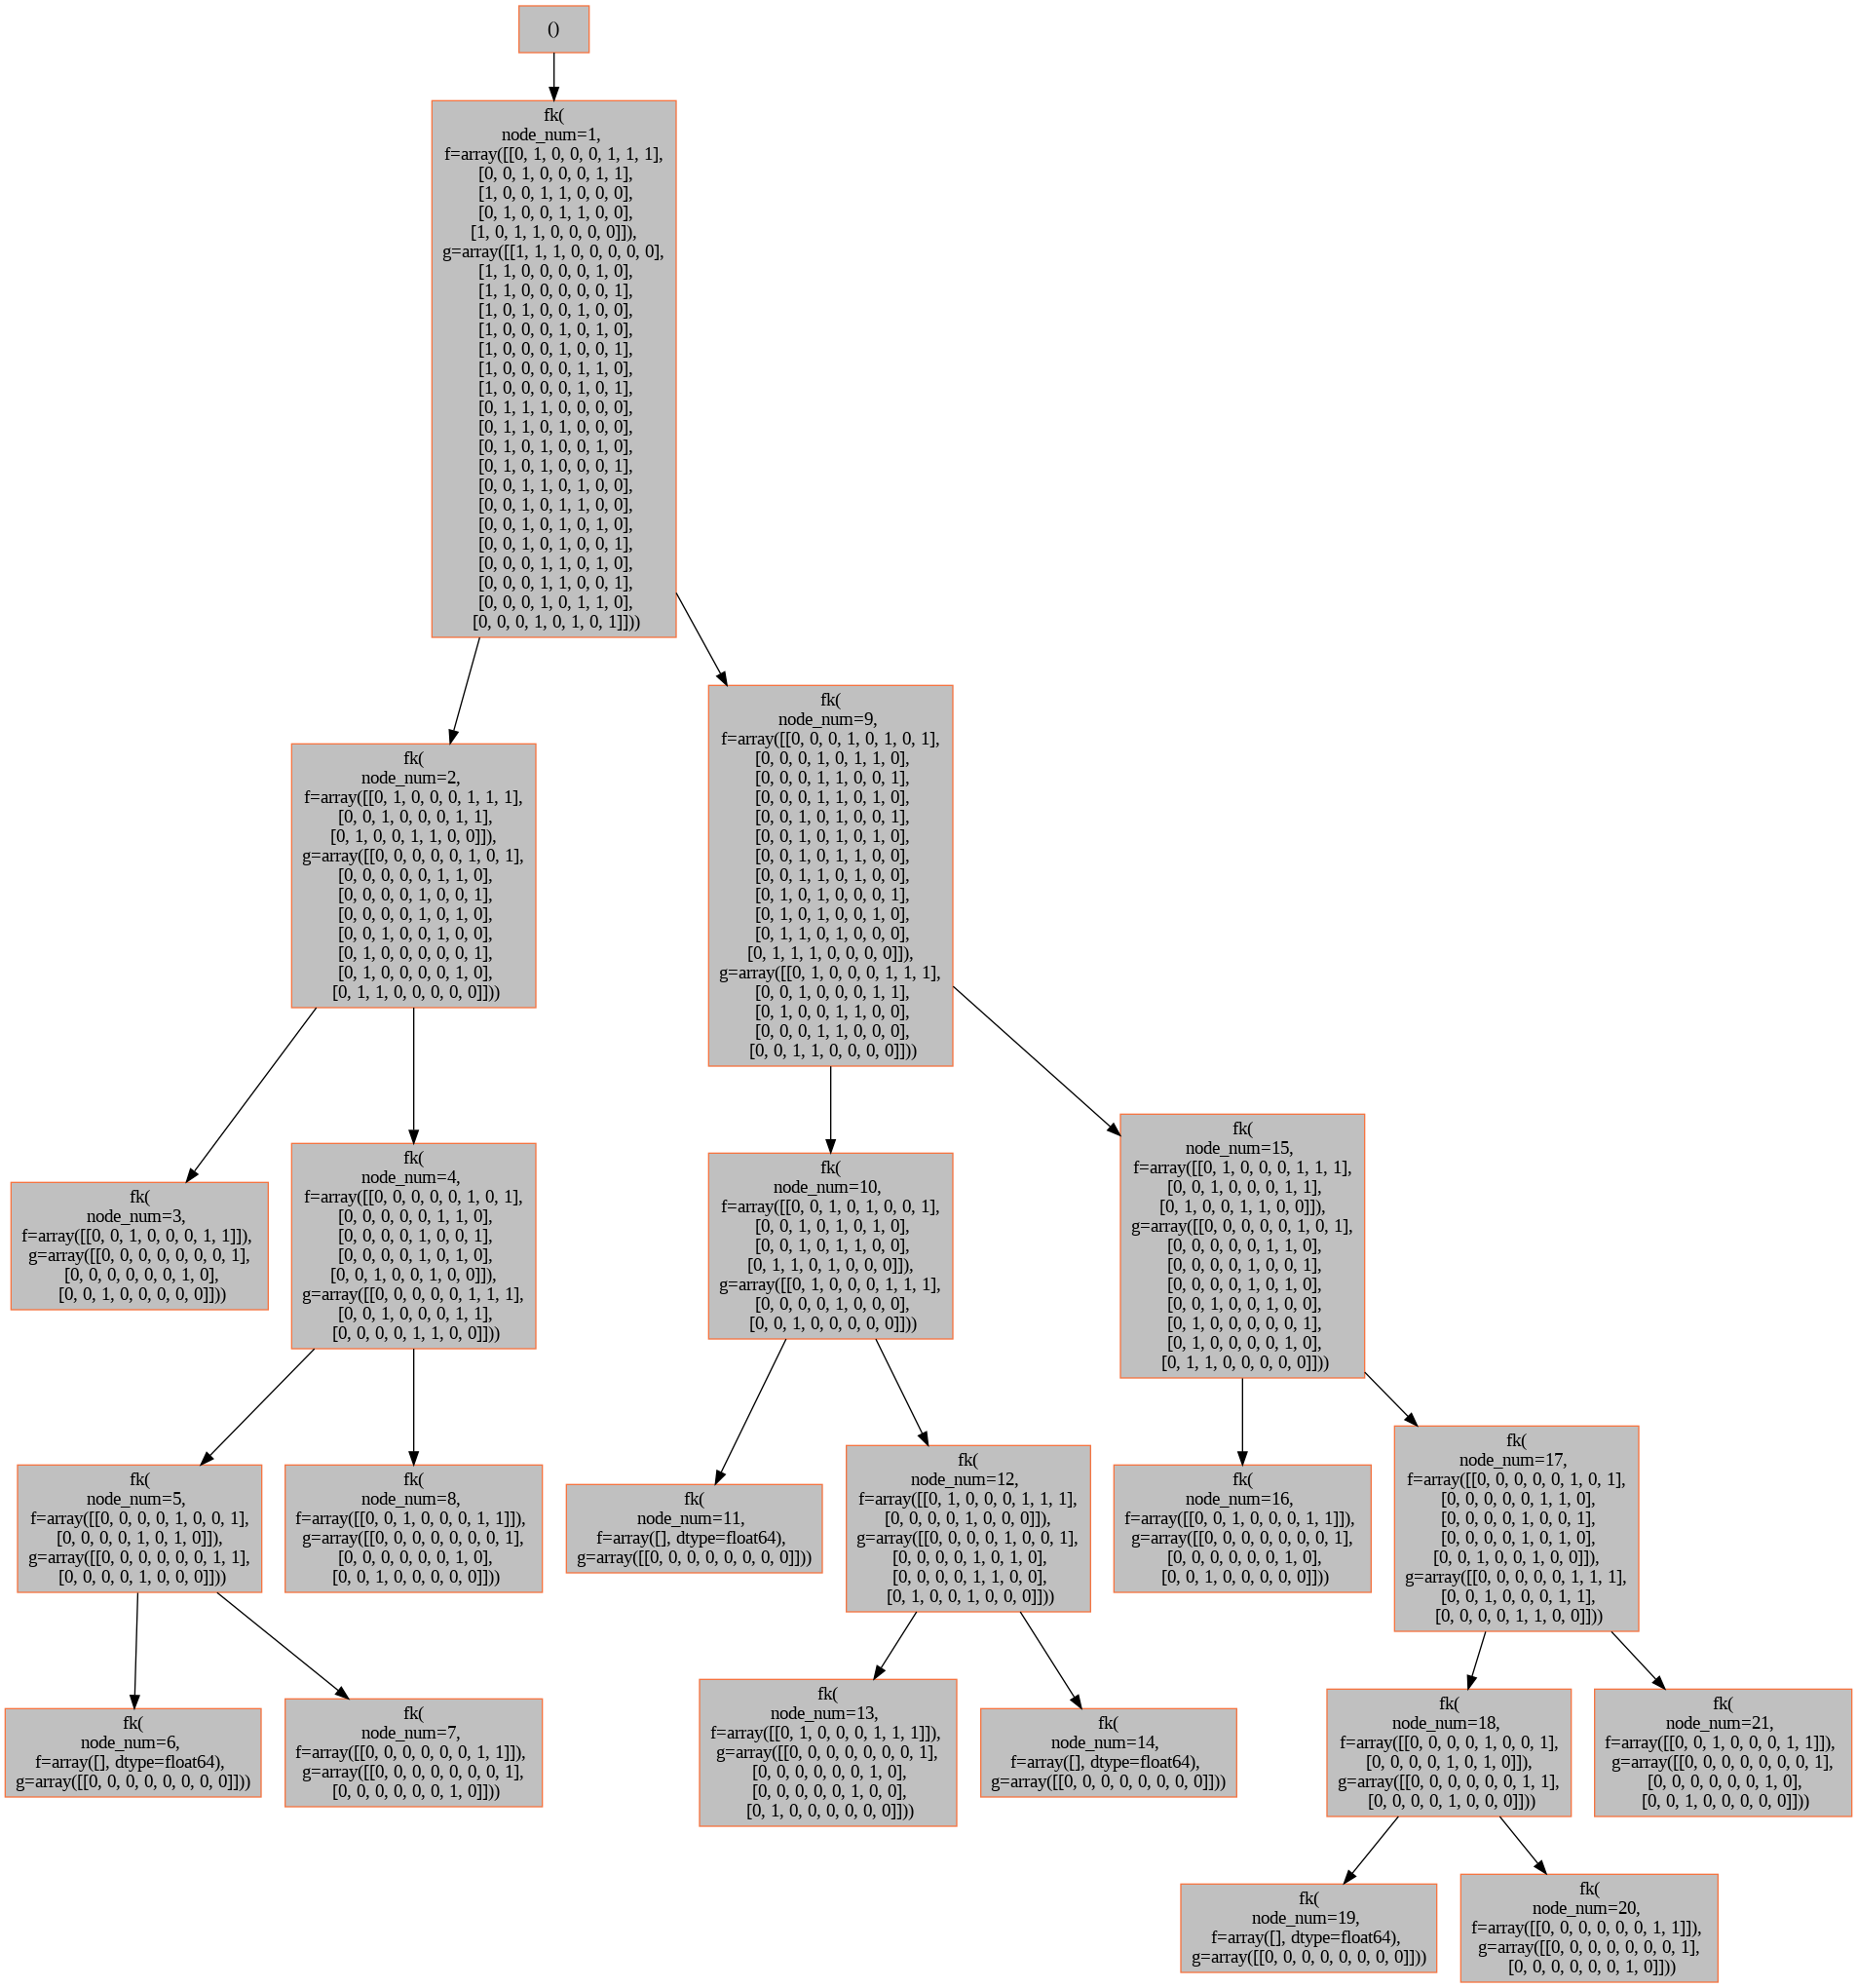
\includegraphics[width=0.62\linewidth]{figures/8ver-fka.png}
\caption{Figures/8Var in\FKA.png}
\end{subfigure}
\caption{\FKA{} recursion tree and automorphism tree of 8-ver. hypergraph}
\end{figure}

\begin{figure}[p]
\centering
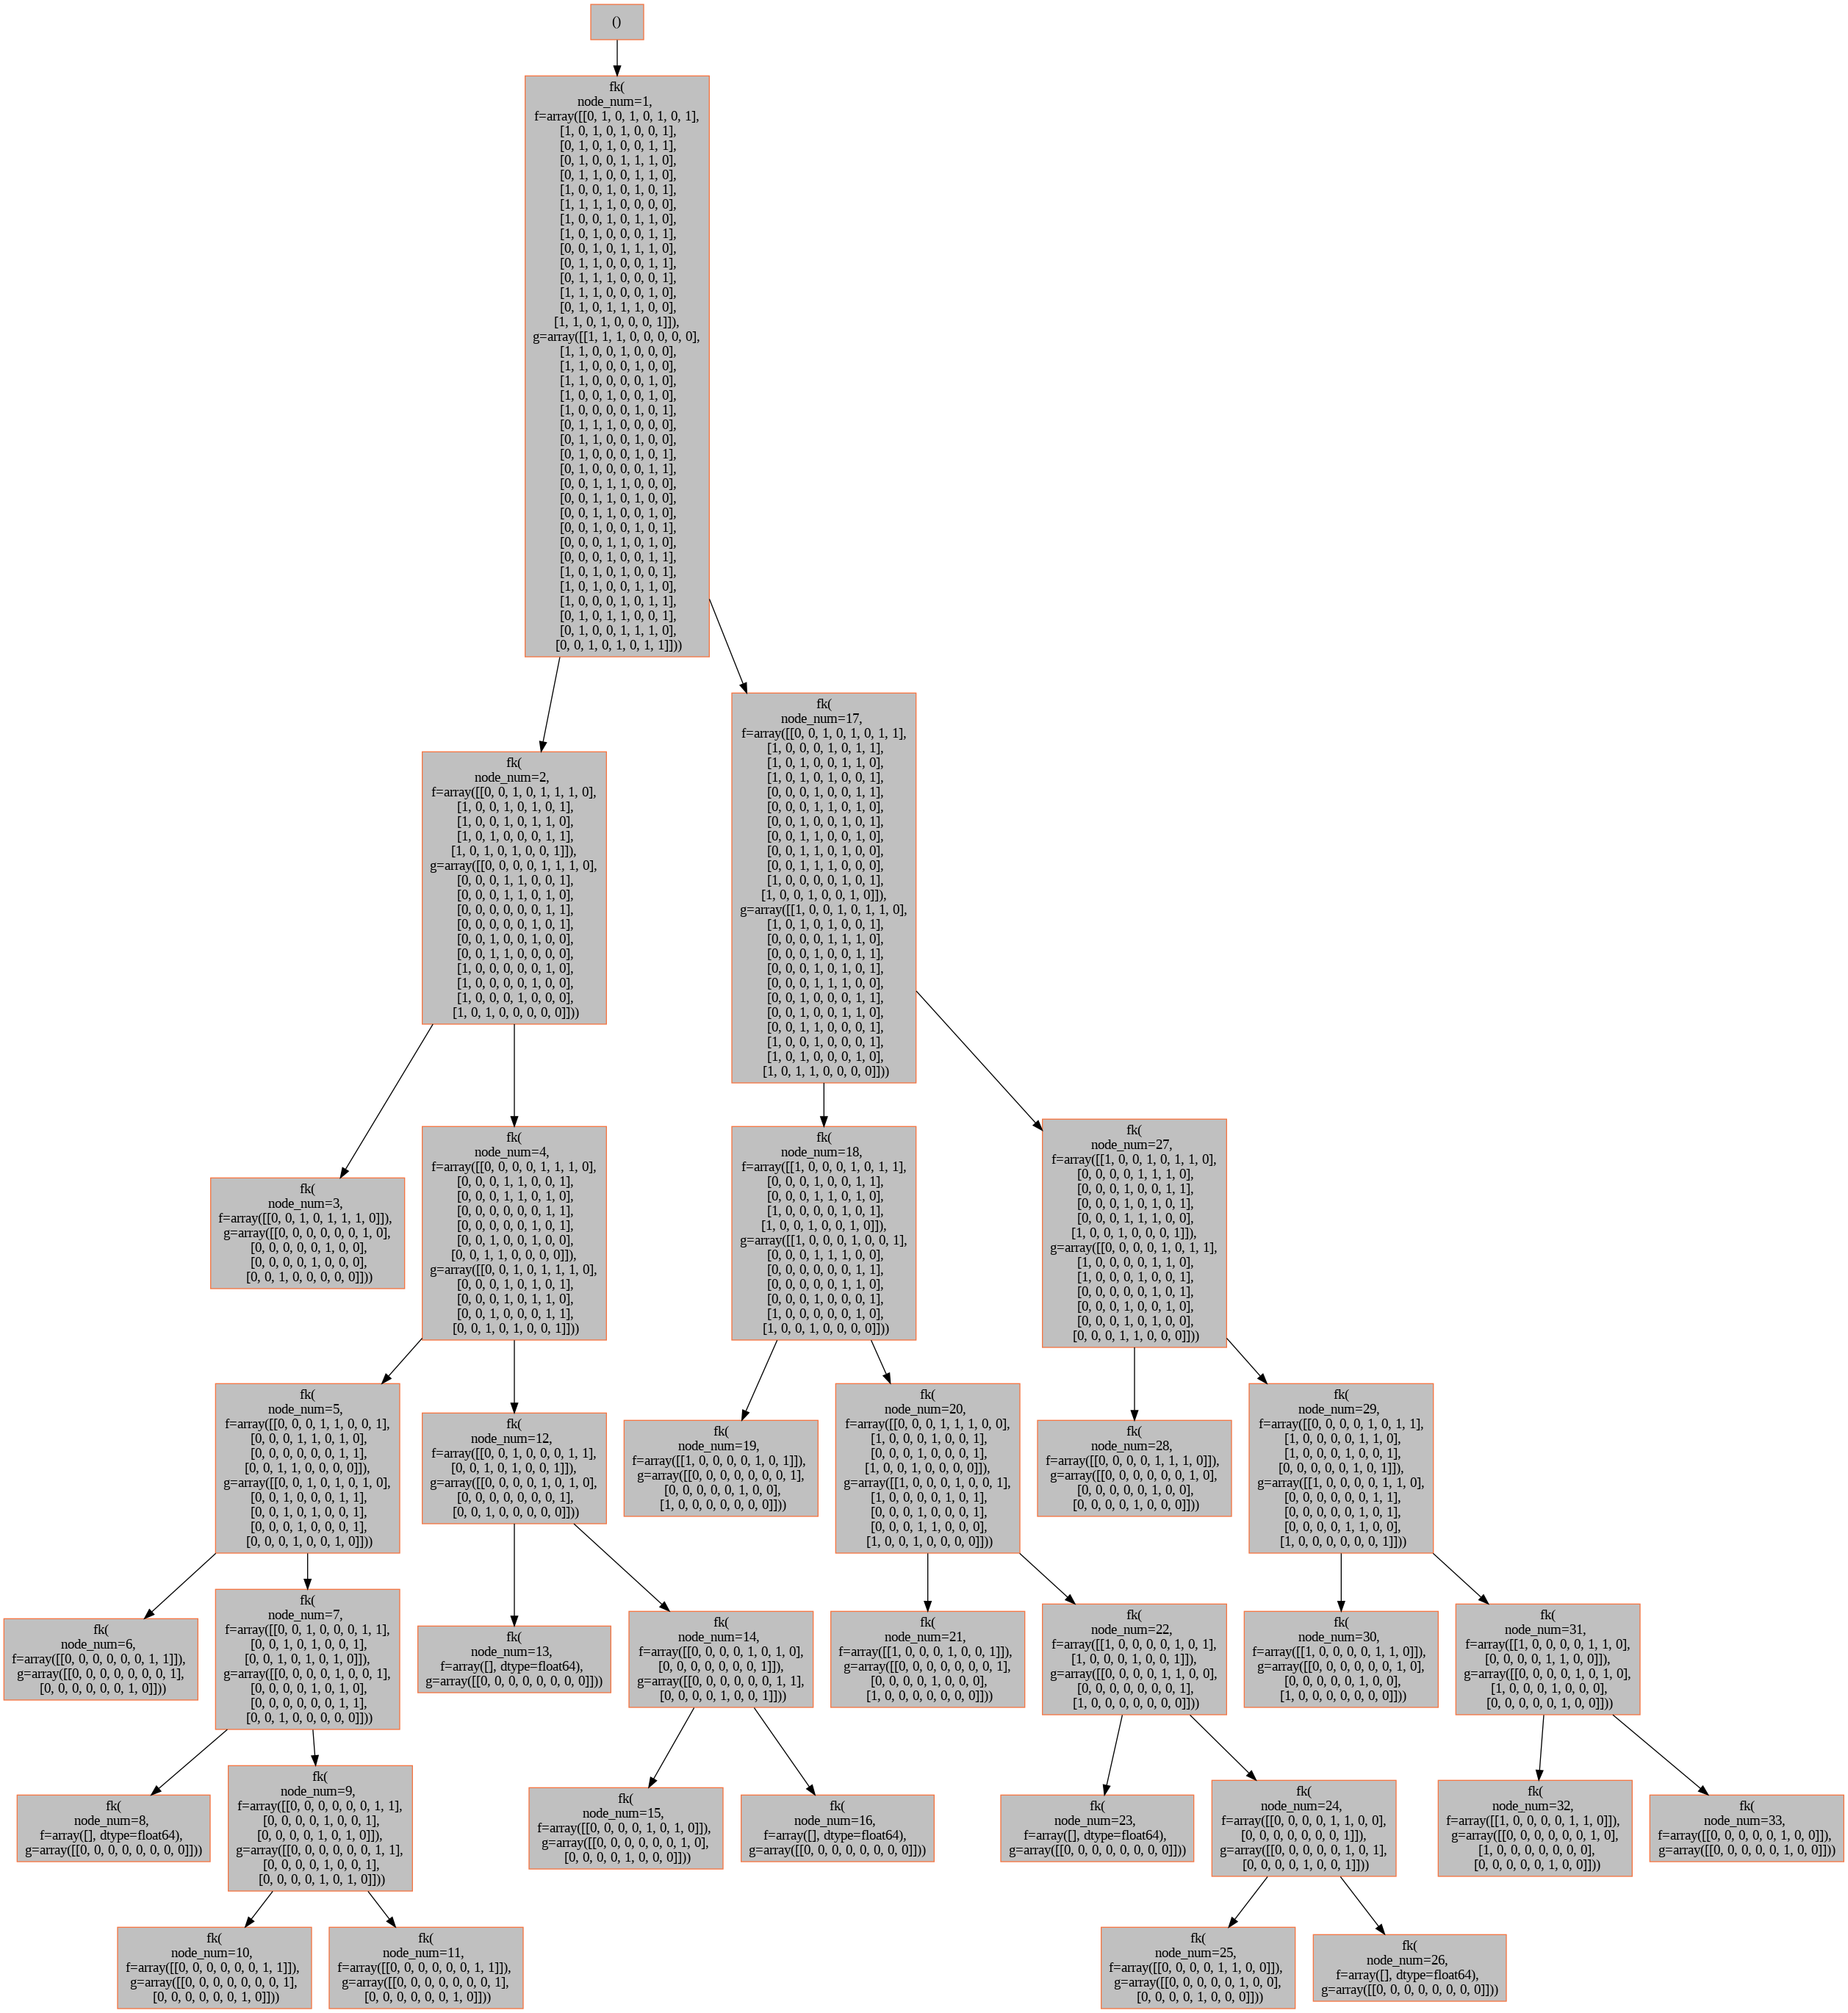
\includegraphics[width=0.75\linewidth]{figures/asym1-fka.png}
\caption{\FKA{} recursion tree on asymmetric hypergraph $Asym_1$}
\end{figure}

\begin{figure}[p]
\centering
\resizebox{\linewidth}{!}{\begin{forest}
autotree
[{\anode{1}{$v_{2}$}{$\text{Trivial}$}{}{Cograph, Chordal}}
  [{\anode{2}{$v_{8}$}{$C_2$}{}{Chordal, Cograph}}
    [{\anode{3}{}{$S_4$}{}{}}]
    [{\anode{4}{$v_{1}$}{$C_2\times C_2$}{}{Chordal, Cograph}}
      [{\anode{5}{$v_{7}$}{$C_2\times C_2$}{ROH, $\alpha$-acyclic}{}}
        [{\anode{6}{}{$C_2$}{}{}}]
        [{\anode{7}{$v_{4}$}{$C_2\times C_2$}{ROH, $\alpha$-acyclic}{}}
          [{\anode{8}{}{$\{\}$}{}{}}]
          [{\anode{9}{$v_{6}$}{$C_2$}{}{}}
            [{\anode{10}{}{$C_2$}{}{}}]
            [{\anode{11}{}{$\{\}$}{}{}}]
          ]
        ]
      ]
      [{\anode{12}{$v_{3}$}{$C_2\times C_2$}{}{Chordal, Cograph}}
        [{\anode{13}{}{$S_3$}{}{}}]
        [{\anode{14}{$v_{4}$}{$D_4$}{ROH, $\alpha$-acyclic}{}}
          [{\anode{18}{}{$C_2$}{}{}}]
          [{\anode{15}{$v_{6}$}{$C_2$}{}{}}
            [{\anode{16}{}{$\{\}$}{}{}}]
            [{\anode{17}{}{$C_2$}{}{}}]
          ]
        ]
      ]
    ]
  ]
  [{\anode{19}{$v_{1}$}{$\text{Trivial}$}{}{Cograph, Chordal}}
    [{\anode{20}{$v_{4}$}{$C_2$}{$\alpha$-acyclic}{}}
      [{\anode{21}{}{$S_3$}{}{}}]
      [{\anode{22}{$v_{8}$}{$C_2$}{}{}}
        [{\anode{23}{}{$\{\}$}{}{}}]
        [{\anode{24}{}{$C_2$}{}{}}]
      ]
    ]
    [{\anode{25}{$v_{7}$}{$\text{Trivial}$}{}{Cograph, Chordal}}
      [{\anode{26}{$v_{3}$}{$C_2\times C_2$}{}{Cograph, Chordal}}
        [{\anode{27}{}{$S_4$}{}{}}]
        [{\anode{28}{$v_{5}$}{$C_2$}{ROH, $\alpha$-acyclic}{}}
          [{\anode{29}{}{$C_1$}{}{}}]
          [{\anode{30}{}{$S_3$}{}{}}]
        ]
      ]
      [{\anode{31}{$v_{8}$}{$C_2\times C_2$}{ROH, $\alpha$-acyclic}{}}
        [{\anode{32}{$v_{5}$}{$C_2\times C_2$}{ROH, $\alpha$-acyclic}{}}
          [{\anode{33}{}{$\{\}$}{}{}}]
          [{\anode{34}{$v_{6}$}{}{}{}}
            [{\anode{35}{}{$C_2$}{}{}}]
            [{\anode{36}{}{$\{\}$}{}{}}]
          ]
        ]
        [{\anode{37}{}{$C_2$}{}{}}]
      ]
    ]
  ]
]
\end{forest}
}
\caption{Automorphism Tree of an asymmetric hypergraph \textbf{Asym}-1 in \FKA}
\end{figure}

\begin{figure}[p]
\centering
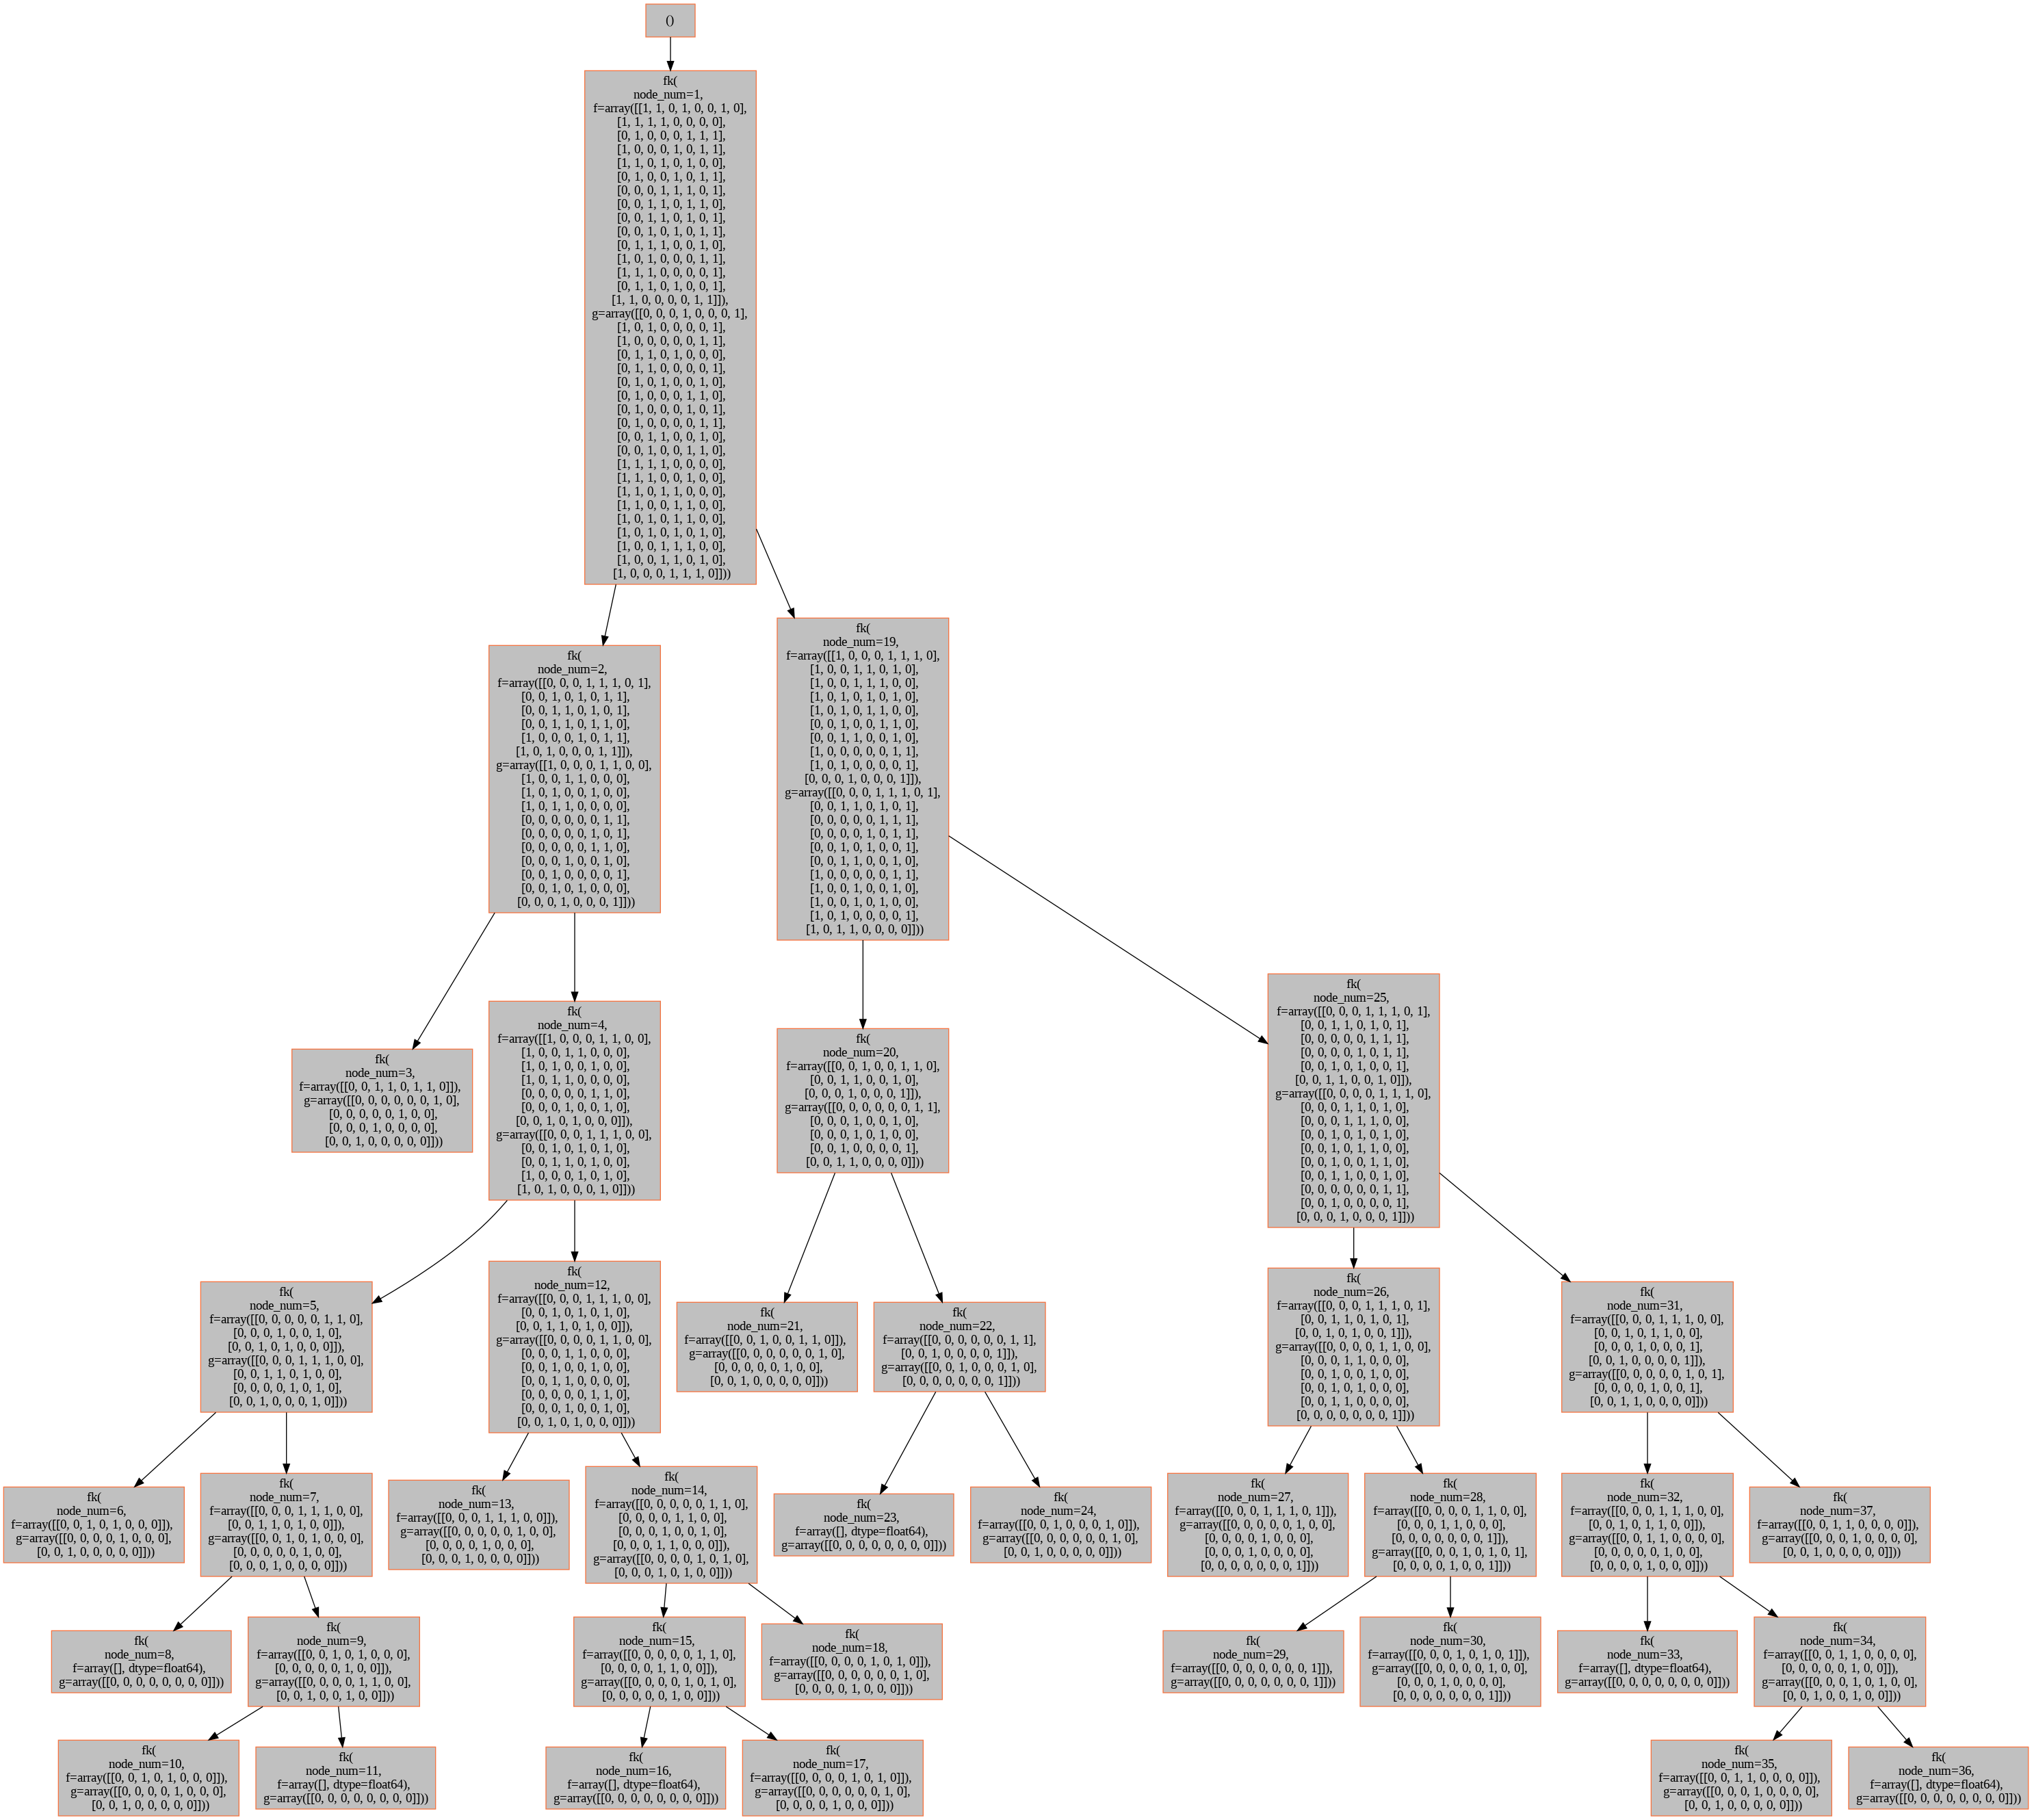
\includegraphics[width=0.9\linewidth]{figures/asym2-fka.png}
\caption{\FKA{} recursion tree on asymmetric hypergraph $Asym_2$}
\end{figure}

\begin{figure}[p]
\centering
\resizebox{\linewidth}{!}{\begin{forest}
autotree
[{\anode{1}{$v_{2}$}{$\text{Trivial}$}{}{Cograph, Split, Chordal}}
  [{\anode{2}{$v_{1}$}{$\text{Trivial}$}{}{Split, Cograph, Chordal}}
    [{\anode{3}{}{$S_4$}{}{}}]
    [{\anode{4}{$v_{6}$}{$\text{Trivial}$}{}{Split, Cograph, Chordal}}
      [{\anode{5}{$v_{4}$}{$C_2$}{}{Split, Cograph, Chordal}}
        [{\anode{6}{}{$C_2$}{}{}}]
        [{\anode{7}{$v_{3}$}{$S_3$}{}{$K_3$}}
          [{\anode{8}{}{$\{\}$}{}{}}]
          [{\anode{9}{$v_{5}$}{$C_3$}{}{$K_3$}}
            [{\anode{10}{}{$C_2$}{}{}}]
            [{\anode{11}{}{$C_2$}{}{}}]
          ]
        ]
      ]
      [{\anode{12}{$v_{3}$}{$C_2\times C_2$}{ROF, $\alpha$-acyclic}{Split}}
        [{\anode{13}{}{$\{\}$}{}{}}]
        [{\anode{14}{$v_{8}$}{$C_2$}{}{}}
          [{\anode{16}{}{$\{\}$}{}{}}]
          [{\anode{15}{}{$C_2$}{}{}}]
        ]
      ]
    ]
  ]
  [{\anode{17}{$v_{3}$}{$\text{Trivial}$}{}{Cograph, Split, Chordal}}
    [{\anode{18}{$v_{7}$}{$C_2$}{}{Cograph, Split, Chordal}}
      [{\anode{19}{}{$S_3$}{}{}}]
      [{\anode{20}{$v_{4}$}{$C_2$}{}{Cograph, Split, Chordal}}
        [{\anode{21}{}{$S_3$}{}{}}]
        [{\anode{22}{$v_{1}$}{$C_2\times C_2$}{$\alpha$-acyclic, Read-Once}{}}
          [{\anode{23}{}{$\{\}$}{}{}}]
          [{\anode{24}{$v_{8}$}{$C_2$}{}{}}
            [{\anode{25}{}{$C_2$}{}{}}]
            [{\anode{26}{}{$\{\}$}{}{}}]
          ]
        ]
      ]
    ]
    [{\anode{27}{$v_{4}$}{$\text{Trivial}$}{}{Cograph, Weakly Chordal}}
      [{\anode{28}{}{$S_3$}{}{}}]
      [{\anode{29}{$v_{8}$}{$C_2$}{}{Split, Cograph, Chordal}}
        [{\anode{30}{}{$S_3$}{}{}}]
        [{\anode{31}{$v_{5}$}{$C_2$}{ROF, $\alpha$-acyclic}{Split}}
          [{\anode{32}{}{$S_3$}{}{}}]
          [{\anode{33}{}{$C_1$}{}{}}]
        ]
      ]
    ]
  ]
]
\end{forest}
}
\caption{Automorphism Tree of an asymmetric hypergraph \textbf{Asym}-2in \FKA}
\end{figure}
